%%%%%%%%%%%%%%%%%%%%%%%%%%%%%%%%%%%%%%%%%%%%%%%%%%%%%%%%%%%%%%%%%
%                                                               %
%                       Legal Notice                            %
%                                                               %
% This document is copyright (C) Jason Gobat & Darren Atkinson	%
%                                                               %
%%%%%%%%%%%%%%%%%%%%%%%%%%%%%%%%%%%%%%%%%%%%%%%%%%%%%%%%%%%%%%%%%

\newpage{\pagestyle{empty}\cleardoublepage}

\chapter{\felt{} Analysis Types}
\label{analysis}

\def\trans#1{#1^{\rm T}}

\section{Introduction}

Our intent in writing this chapter was to give some basic details on the
kinds of analyses that are intrinsic to \felt{}.  It is not at all meant to
be an introduction to the finite element method, but rather it is meant
to provide a background on what types of physical and mathematical models
we are talking about when we talk about the various analysis types.
There is of course some very basic information on just how these models
work in the context of FEA, but we really do suggest that you try 
some of the excellent textbooks (~\cite{hughes:fem, zienk:taylor:fem,
logan:fem, burnett:fea, segerlind:fea})
that are out there if you want any sort of real background information.

\section{Static structural analysis}

The basic equation for static structural analysis can be seen as a
generalization of Hooke's law for the deformation of a linear spring,
$f = kx$.  For a spring, if we know the applied force and the spring stiffness,
$k$, then we can find the deformation as $x = f/k$.  We can generalize this
to multiple degrees of freedom by considering the static equilibrium of
the general spring in figure~\ref{analysis.spring}.
%
\begin{figure}
 \begin{center}
   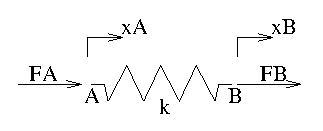
\includegraphics[width=3in]{figures/spring}
 \end{center}
 \caption{Static equilibrium of a general linear spring.}
 \label{analysis.spring}
\end{figure} 
%
If the spring is in static equilibrium then at point a we must have
\begin{equation}
{\left( x_{a} - x_{b} \right) k} = {F_{a}},
\end{equation}
and at point b
\begin{equation}
{\left( x_{b} - x_{a} \right) k} = {F_{b}}.
\end{equation}
These two conditions form a linear system of equations in two unknowns.  We
can rewrite this system in matrix notation as
\begin{equation}
\left[\matrix{
k & -k \cr
-k & k \cr
}\right] 
\left[\matrix{
x_{a} \cr
x_{b} \cr
}\right] =
\left[\matrix{
F_{a} \cr
F_{b} \cr
}\right].
\label{spring_stiffness}
\end{equation}
The problem is still essentially the same as our simple Hooke's law
calculation -- we know the applied force and the structural stiffness, and
we want to solve for the deformations.  Now, however, our applied force is
a vector, our structural stiffness is a matrix and to solve for the
deformations we must now solve a linear system of equations.

The {\em stiffness matrix} on the left hand side of 
equation~\ref{spring_stiffness} is
just the element stiffness matrix in the finite element method.  When we
want to solve a problem of static equilibrium for a structure that
is more complex than our simple spring all we have to do is stick a bunch
of springs together and then linearly superpose the contributions
from each element's stiffness matrix into our {\em global} stiffness matrix.
Consider the case of two springs in series as in figure~\ref{analysis.spring2}.
%
\begin{figure}
 \begin{center}
  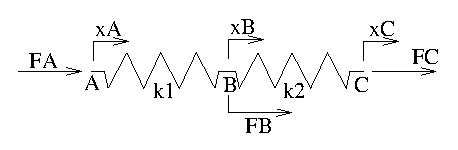
\includegraphics[width=3.5in]{figures/spring2}
 \end{center}
 \caption{Static equilibrium of two springs in series.}
 \label{analysis.spring2}
\end{figure} 
%
Each individual spring has a stiffness matrix like the one on the left hand
side of equation~\ref{spring_stiffness}.  The system now has three
degrees of freedom ($x_a$, $x_b$, $x_c$) and thus we know that our global
stiffness matrix will be $3 \times 3$.  We assemble the global stiffness
matrix (construct the superposition of all the element stiffness matrices)
by considering which degrees of freedom each spring affects -- spring 1
affects the deformations $x_a$ and $x_b$; spring 2 affects $x_b$ and $x_c$.
We know then that the stiffness at b in our global stiffness matrix
will have contributions from both spring 1 and spring 2.  The global
stiffness matrix is
\begin{equation}
\def\tempa#1{\multicolumn{1}{|c}{#1}}
\def\tempb#1{\multicolumn{1}{c|}{#1}}
\def\tempc#1{\multicolumn{1}{|c|}{#1}}
{K} = 
{\left[\begin{array}{ccc}
\cline{1-2}
\tempa{k_{1}}  & \tempb{-k_{1}}        & 0     \\ \cline{2-3}
\tempa{-k_{1}} & \tempc{k_{1} + k_{2}} & \tempb{-k_{2}} \\ \cline{1-2}
0      & \tempa{-k_{2}}        & \tempb{k_{2}} \\ \cline{2-3}
\end{array}\right]}.
\end{equation}
The two boxes indicate exactly how the individual element stiffness matrices
were placed into the global stiffness matrix.  Our equation for static
equilibrium is
\begin{equation}
\left[\matrix{
k_{1}  & -k_{1}        & 0 \cr
-k_{1} & k_{1} + k_{2} & -k_{2} \cr
0      & -k_{2}        & k_{2} \cr
}\right] 
\left[\matrix{
x_{a} \cr
x_{b} \cr
x_{c} \cr
}\right] =
\left[\matrix{
F_{a} \cr
F_{b} \cr
F_{c} \cr
}\right].
\label{spring_equilibrium}
\end{equation}

Of course, one-dimensional springs are not the most useful element in
terms of modeling complex structural behavior.  The concepts of 
static equilibrium, superposition, and assembly, however, are identical no 
matter what types of elements we are using.  All that changes the is nature of 
the element stiffness matrices -- rather than simple linear springs we take into 
account bending and torsional stiffness, three-dimensional solid deformations,
plate bending motion, etc.    In structural analysis there are only six
possible degrees of freedom (translations along and rotations about the
x, y, and, z axes) and thus if we know how each element affects
each of these degrees of freedom we can even mix different element types
into the same global stiffness matrix.  Given a global stiffness matrix, $K$,
which represents the contributions from an arbitrary number of individual
elements and a vector, $F$, of the force at each global degree of
freedom, then the general form of equation~\ref{spring_equilibrium} is simply
\begin{equation}
Kx = F
\end{equation}
where $x$ is a vector of the displacements at each global degree of freedom
which we solve for using matrix techniques for linear systems of equations.
Note the direct analogy between this matrix equation and the simple linear
spring relationship, \mbox{$f = kx$}, cited earlier.

\section{Transient structural analysis}

Just like static structural analysis is an extension of simple static
equilibrium for a spring, we can draw an analogy between dynamic structural
analysis and a simple spring-mass-dashpot oscillator.  For the system
shown in figure~\ref{spring_mass}, a sum of forces at the mass and
%
\begin{figure}
 \begin{center}
  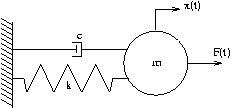
\includegraphics[width=4in]{figures/spring_mass}
 \end{center}
 \caption{Dynamic equilibrium of a spring-mass-dashpot system.}
 \label{spring_mass}
\end{figure} 
%
Newton's law gives
\begin{equation}
{m {\ddot x} + c {\dot x} + k x} = f(t)
\end{equation}
where the overdot indicates differentiation in time.  To generalize this
to multiple degrees of freedom we take the same steps as in the static
case, recognizing that we can assemble global mass and damping matrices
from elemental constructs just as we did for the stiffness matrix in the
static case.  In that case, the matrix equation of motion becomes
\begin{equation}
{M {\ddot x} + C {\dot x} + K x} = F(t)
\label{matrix_motion}
\end{equation}
where $M$, $C$, and $K$ are now global mass, damping and stiffness matrices,
$x$ is a vector of displacements at each DOF just as before and $F(t)$
is a time-dependent vector of forces at each degree of freedom.

The damping matrix is the most difficult quantity to estimate in 
equation~\ref{matrix_motion}; both the stiffness and mass matrices are
relatively simple to derive for a wide variety of elements (see 
chapter~\ref{elements}).  There is no explicit way to specify dashpot
constants in \felt{}.  Instead, damping is based on a Rayleigh model
whereby the damping matrix is simply a linear combination of the
mass and stiffness matrices
\begin{equation}
C = {R_{m} M + R_{k} K} 
\end{equation}
where $R_m$ and $R_k$ are user specified constants of proportionality.

\section{Static thermal analysis}

\section{Transient thermal analysis}

% \begin{equation}
% {M {\dot x} + K x} = F(t)
% \end{equation}

\section{Modal analysis}

There are two basic levels to modal analysis.  The first is the eigenvalue
problem which determines the natural frequencies and mode shapes of our
structure in free ($F(t) = 0$), undamped ($C = [0]$) vibration.  If we assume 
a solution to the undamped, unforced form of equation~\ref{matrix_motion} 
of the form
\begin{equation}
{x(t)} = {u {\rm e}^{i \omega t}}
\end{equation}
(where $u$ is a vector of displacement amplitudes) and substitute this
into the equation of motion, we find that
\begin{equation}
{\left[ K - M \omega^{2} \right] u} = 0.
\label{eigenvalue_problem}
\end{equation}
Linear algebra tells us that this has a non-trivial solution only if
\begin{equation}
{\det \left[ K - M \omega^{2} \right]} = 0.
\end{equation}
Evaluating the determinant leads to a polynomial of order $n$ (where $n$
is the number of DOF in the problem) in $\omega^2$.  The roots of this
polynomial give us the free vibration natural frequencies, $\omega_{i}^{2}$,
$i = 1 \ldots n$.  If we substitute each of these $\omega_i$ into
equation~\ref{eigenvalue_problem} we can solve for $n$ mode shape vectors,
$u^{(i)}$.  

By itself, natural frequency and mode shape information can be very useful;
the natural frequencies are an immediate indication of where the resonances
for this system will be (even when we put damping back into the system).
The second level of modal analysis, however, uses the fact that the 
eigenvectors (mode shapes) form an orthogonal basis set to
decouple an arbitrarily complex multiple degree of freedom system into
$n$ single degree of freedom systems.  If we form a matrix, $U$, of all the
eigenvectors, $u^{(i)}$, then we can compute the modal mass and stiffness
matrices as
\begin{eqnarray}
{\hat M} = {\trans{U} M U} \\
{\hat K} = {\trans{U} K U}.
\end{eqnarray}
The modal matrices have the remarkable property that they are diagonal
and thus if we form a transformed system of coordinates,
\begin{equation}
q = {U^{-1} x},
\end{equation}
and a transformed force vector
\begin{equation}
Q = {\trans{U} F},
\end{equation}
we can write our matrix equation of motion as $n$ uncoupled 
single degree of freedom equations
\begin{equation}
{{\hat M}_{i} {\ddot q}_{i} + {\hat K}_{i} q_{i}} = {Q_{i}}, \hspace{0.25in} i = 1 \ldots n.
\end{equation}
We say that ${\hat M}_i$ and ${\hat K}_i$ are the modal mass and stiffness
in the $i$th mode.  They are simple the $i$th entries along the diagonals
of the modal mass and stiffness matrices.  We can further simplify the
resulting equations of motion by making use of the fact that the
eigenvectors can be arbitrarily normalized (they are only fixed to within
an arbitary multiplicative constant by equation~\ref{eigenvalue_problem}).
If we choose an appropriate normalization then we can fix it so that 
${\hat M} = I$, the identity matrix.  The appropriately normalized
mode shapes are called orthonormal modes.

Because \felt{} uses a Rayleigh damping model, we can also construct
a diagonal damping matrix,
\begin{equation}
{\hat C} = {\trans{U} C U} = {R_{m} {\hat M} + R_{k} {\hat K}}.
\end{equation}
Also, because the motion in each mode is now just like a single degree
of freedom motion, we can use concepts from the theory of single
degree of freedom oscillators to help us choose $R_k$ and $R_m$.  The
damping ratio in the $i$th mode is simply
\begin{equation}
{\zeta_{i}} = {{\hat C_{i}} \over {2 {\hat M}_{i} \omega_{i}}}
\label{damping_ratio}
\end{equation}
We can fix the damping ratio in two modes, $i$ and $j$, simply by substituting
\begin{eqnarray}
{{\hat C}_{i}} = {R_{m} {\hat M}_{i} + R_{k} {\hat K}_{i}}, \\
{{\hat C}_{j}} = {R_{m} {\hat M}_{j} + R_{k} {\hat K}_{j}},
\end{eqnarray}
into equation~\ref{damping_ratio} and solving the resulting linear
system for $R_m$ and $R_k$
\begin{equation}
\left[\matrix{
{1 \over \omega_{i}} & \omega_{i} \cr
{1 \over \omega_{j}} & \omega_{j} \cr
}\right] 
\left[\matrix{
R_{m} \cr
R_{k} \cr
}\right] = 
\left[\matrix{
2 \zeta_{i} \cr
2 \zeta_{j} \cr
}\right].
\end{equation}

After solving the $n$ uncoupled single degree of freedom equations 
(either as initial value problems or steady state oscillation problems)
for the individual $q_i$, we can form the solution in physical
coordinates as the superposition of the motion in each mode
\begin{equation}
x(t) = {\sum_{i = 1}^{n} u^{(i)} q_{i}(t)} = Uq.
\end{equation}

\section{Spectral analysis}

Spectral analysis is intended to give us information about the response
of our structural system in the frequency domain.  In a way, we can think
of it as a direct way to calculate the results that we would get from
estimating a power spectrum of our time domain results using a fast
fourier transform.  If we assume that the force vector in 
equation~\ref{matrix_motion} is harmonic in time and of the form,
\begin{equation}
F(t) = {F_{0} {\rm e}^{i \omega t}}
\end{equation}
then we can also assume the solution, $x(t)$, is of the form\footnote{It is
a property of linear systems that the output will always be at the same
frequency as the input.}
\begin{equation}
x(t) = {{\hat x}_{0} {\rm e}^{i \omega t}}.
\end{equation}
Note that ${\hat x}_{0}$ is a complex constant which incorporates both the
magnitude and phase of the output motion
\begin{equation}
{{\hat x}_{0}} = {x_{0} {\rm e}^{-i \phi}}.
\end{equation}
If we differentiate, substitute into equation~\ref{matrix_motion}, and
divide out the time dependent harmonic term then we find that
\begin{equation}
{F_{0}} = {\left[{-\omega^{2} M + i \omega C + K}\right] {\hat x}_{0}}.
\end{equation}
If this were a single degree of freedom system we would recognize the
term in square brackets on the right hand side as the inverse of the
transfer function.  In a multiple degree of freedom system, this term is known
as the impedance matrix,
\begin{equation}
{Z} = -\omega^{2} M + i \omega C + K,
\end{equation}
and its inverse is equivalent to a matrix of single degree of freedom
transfer functions
\begin{equation}
{H} = {Z}^{-1}.
\end{equation}
In essence, the transfer function matrix predicts the amount of response
per unit force at frequency $\omega$. 

Given entries from the transfer function matrix $H_{ij}(\omega)$, we can
calculate the output spectrum at DOF $i$ due to system inputs as
\begin{equation}
{S_{i}^{\rm (out)}} = {\sum_{k = 1}^{n} \left|{H_{ik}(\omega)}\right|^{2} S_{k}^{(in)}},
\end{equation}
where the input spectra $S_{k}^{\rm (in)}$ are simply the power spectra of the
applied forces.

\section{Nonlinear static analysis}

\section{Nonlinear dynamic analysis}
